\documentclass[a4paper]{article}
\usepackage{ucs}  % unicode
\usepackage[utf8x]{inputenc}
% \usepackage[T2A]{fontenc}
% \usepackage[bulgarian]{babel}
\usepackage{graphicx}
% \usepackage{fancyhdr}
% \usepackage{lastpage}
\usepackage{listings}
\usepackage{slashbox}
\usepackage{multirow}
% \usepackage{fancyvrb}
% \usepackage[usenames,dvipsnames]{color}
% \setlength{\headheight}{12.51453pt}

%\pagestyle{fancy}
%\fancyhead{}
%\fancyfoot{}

% \cfoot{\thepage\ от \pageref{LastPage}}

% \addto\captionsbulgarian{%
%   \def\abstractname{%
%     Цел на проекта} %\cyr\CYRA\cyrs\cyrt\cyrr\cyra\cyrk\cyrt}}%
% }

% Custom defines:
\def\definition{Definition:\ }
\def\la{\leftarrow}
\def\vars{\mathrm{Vars}}
\def\occ{\mathrm{Occ}}
% \def\dc{bar baz}

% TODO remove colorlinks before printing
% \usepackage[unicode,colorlinks]{hyperref}   % this has to be the _last_ command in the preambule, or else - no work
% \hypersetup{urlcolor=blue}
% \hypersetup{citecolor=PineGreen}

\begin{document}

\newcommand{\aee}[1] {[[#1]]^\sharp}
\newcommand{\cc}[1] {\texttt{#1}}
% 1.Подробно математическо описание на алгоритъма
% 2. Описание на работата на програмата с примери, разпечатка на кода,
% подробен user guide. Кодът трябва да е написан ясно и четливо, с подходящи коментари
% 3. Кривите да се чертаят като се използва алгоритъма на de Casteljau

% \title{\rbc}
% \author{
% Зорница Атанасова Костадинова, 4 курс, КН, фн: 80227
% }
% \date{\today}
% \maketitle
% 
% %\includegraphics[scale=0.1]{drop}
% 
% \begin{abstract}
% Настоящият документ е курсова работа към проекта ``\rbc'' по предмета ``Компютърно геометрично моделиране''. Описан е математическият алгоритъм за пресмятане на кривата. Обяснена е програмната реализация на проекта.
% \end{abstract}
% \newpage
% 
% \setcounter{tocdepth}{2}
% \tableofcontents
% \newpage

\title{Static Program Analysis - Exercise 1}
\author{Iskren Ivov Chernev \\ tutorial group B}

\maketitle

\begin{enumerate}
  \item \em{}Solution\em

  \vspace{5mm}

  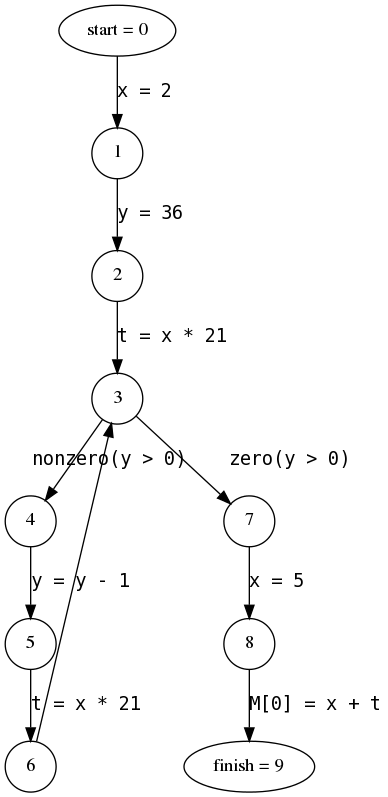
\includegraphics[scale=0.3]{1-1a.png}
  \hspace{2cm}
  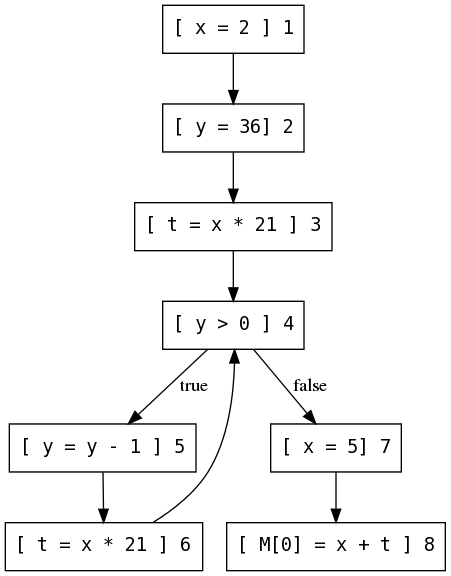
\includegraphics[scale=0.4]{1-1b.png}

  \item \em{}Solution\em \\
  
  Let $ \mathrm{Expr} $ be the set of all expressions containing variables.

  We will define the abstract edge effect $ [[k]]^\sharp $: a function which
  transforms the available expressions before a label to the available
  expressions after that label (i.e. it shows how each label acts on the set of
  available expressions).
  Let $ A \subseteq 2^{\mathrm{Expr}} $ be the set of available expressions,
  before the execution of label $ lab $. Then:
  \begin{itemize}
    \item $ [[;]]^\sharp A = A $
    \item $ [[NonZero(e)]]^\sharp A = [[Zero(e)]]^\sharp A = A \cup \{ e \} $
    \item $ [[x \la e]]^\sharp A = [[x \la M[e]\;]]^\sharp A = (A \cup \{ e \}) \setminus \occ(x) $ \\ where $ \occ(x) = \{ e'\ |\ x \in \vars(e') \} $
    \item $ [[M[e_1] \la e_2]]^\sharp = A \cup \{ e_1, e_2 \} $
  \end{itemize}
  Note: We never add expressions consisting of constant values. \\ Because
  $ [[k]]^\sharp $ are regular functions acting on sets, we can combine them
  (with function composition) to obtain the path effect along any given path.
  Let $ \pi = k_0 k_1 \dots k_n $ is a path of execution. Then the abstract
  effect of the path $ \pi $ is defined by:

  $$ [[\pi]]^\sharp = \aee{k_n} \circ \aee{k_{n-1}} \circ \dots \circ \aee{k_2} \circ \aee{k_1} $$

  We can obtain the set of available assignments at the end of $ \pi $ by
  applying the abstract path effect to the empty set (because initially there
  are no available expressions).

  $$ \aee{\pi} \emptyset = \aee{k_n}(\aee{k_{n-1}}(\dots\aee{k_2}(\aee{k_1}\emptyset)\dots)) $$

  Finally, we should define the available expressions at a particular program
  point $ v $. To do this we need to combine all paths $ \pi $ that start from
  the program beginning and end at $ v $. The combination is done with \em set
  intersection \em, because an expression is available at a particular point only
  if it is available at the end of all paths leading to that program point.

  $$ \mathcal{A}^\star[v] = \bigcap \{ \aee{\pi} \emptyset\ |\ \pi = \mbox{start } k_1 \dots k_{n-1}\ v \} $$

  \item Solution \\

  System of inequalities:

  \begin{eqnarray*}
    \mathcal{A}[0] &\subseteq& \emptyset \\
    \mathcal{A}[1] &\subseteq& \mathcal{A}[0] \setminus \occ(x) \\
    \mathcal{A}[2] &\subseteq& \mathcal{A}[1] \setminus \occ(y) \\
    \mathcal{A}[3] &\subseteq& \mathcal{A}[2] \cup \{ \cc{x * 21} \} \setminus \occ(t) \\
    \mathcal{A}[3] &\subseteq& \mathcal{A}[6] \\
    \mathcal{A}[4] &\subseteq& \mathcal{A}[3] \cup \{ \cc{y > 0} \} \\
    \mathcal{A}[5] &\subseteq& \mathcal{A}[4] \cup \{ \cc{y - 1} \} \setminus \occ(y) \\
    \mathcal{A}[6] &\subseteq& \mathcal{A}[5] \cup \{ \cc{x * 21} \} \setminus \occ(t) \\
    \mathcal{A}[7] &\subseteq& \mathcal{A}[3] \cup \{ \cc{y > 0} \} \\
    \mathcal{A}[8] &\subseteq& \mathcal{A}[7] \setminus \occ(x) \\
    \mathcal{A}[9] &\subseteq& \mathcal{A}[8] \cup \{ \cc{x + t} \} \\
  \end{eqnarray*}

  Maximal (set inclusion), least (lattice theory) solution:

  \begin{tabular}{lll}
    $\mathcal{A}[0]$ & = & $\emptyset$                     \\
    $\mathcal{A}[1]$ & = & $\emptyset$                     \\
    $\mathcal{A}[2]$ & = & $\emptyset$                     \\
    $\mathcal{A}[3]$ & = & $\{\cc{x * 21}\}$               \\
    $\mathcal{A}[4]$ & = & $\{\cc{x * 21}, \cc{y > 0}\}$   \\
    $\mathcal{A}[5]$ & = & $\{\cc{x * 21}\}$               \\
    $\mathcal{A}[6]$ & = & $\{\cc{x * 21}\}$               \\
    $\mathcal{A}[7]$ & = & $\{\cc{x * 21}, \cc{y > 0}\}$   \\
    $\mathcal{A}[8]$ & = & $\{\cc{y > 0}\}$                \\   
    $\mathcal{A}[9]$ & = & $\{\cc{x + t}, \cc{y > 0}\}$    \\
  \end{tabular}

  % We will solve the system of inequalities using the iteration method.

  % \begin{tabular}{|l|*{6}{l|}}
  %   \hline
  %   \backslashbox{$\mathcal{A}[i]$}{iter} &
  %                      0           & 1                 & 2                 & 3                             & 4                             & 5                      \\
  %   \hline
  %   $\mathcal{A}[0]$ & $\emptyset$ & $\emptyset$       & $\emptyset$       & $\emptyset$                   & $\emptyset$                   & \multirow{10}{*}{done} \\
  %   $\mathcal{A}[1]$ & $\emptyset$ & $\emptyset$       & $\emptyset$       & $\emptyset$                   & $\emptyset$                   &                        \\
  %   $\mathcal{A}[2]$ & $\emptyset$ & $\emptyset$       & $\emptyset$       & $\emptyset$                   & $\emptyset$                   &                        \\
  %   $\mathcal{A}[3]$ & $\emptyset$ & $\emptyset$       & $\{\cc{x * 21}\}$ & $\{\cc{x * 21}\}$             & $\{\cc{x * 21}\}$             &                        \\
  %   $\mathcal{A}[4]$ & $\emptyset$ & $\{\cc{y > 0}\}$  & $\{\cc{y > 0}\}$  & $\{\cc{x * 21}, \cc{y > 0}\}$ & $\{\cc{x * 21}, \cc{y > 0}\}$ &                        \\
  %   $\mathcal{A}[5]$ & $\emptyset$ & $\emptyset$       & $\emptyset$       & $\emptyset$                   & $\{\cc{x * 21}\}$             &                        \\
  %   $\mathcal{A}[6]$ & $\emptyset$ & $\{\cc{x * 21}\}$ & $\{\cc{x * 21}\}$ & $\{\cc{x * 21}\}$             & $\{\cc{x * 21}\}$             &                        \\
  %   $\mathcal{A}[7]$ & $\emptyset$ & $\{\cc{y > 0}\}$  & $\{\cc{y > 0}\}$  & $\{\cc{x * 21}, \cc{y > 0}\}$ & $\{\cc{x * 21}, \cc{y > 0}\}$ &                        \\
  %   $\mathcal{A}[8]$ & $\emptyset$ & $\emptyset$       & $\{\cc{y > 0} \}$ & $\{\cc{y > 0}\}$              & $\{\cc{y > 0}\}$              &                        \\
  %   $\mathcal{A}[9]$ & $\emptyset$ & $\{\cc{x + t}\}$  & $\{\cc{x + t}\}$  & $\{\cc{x + t}, \cc{y > 0}\}$  & $\{\cc{x + t}, \cc{y > 0}\}$  &                        \\
  %   \hline
  % \end{tabular}

  \item Solution \\

  % \definition A not available expression is an expression, which has not been
  % computed or whose whose constituent variables have been changed after its
  % computation.

  Let $ \mathrm{Expr} $ be the set of all expressions containing variables.

  We will define the abstract edge effect $ [[k]]^\sharp $ showing how each
  edge (label) transforms the set of non available expressions before it to the
  set of non available expressions after it. \\
  Let $ N \subseteq 2^{\mathrm{Expr}} $ be the set of not available
  expressions, before the execution of label $ lab $. Then:
  \begin{itemize}
    \item $ [[;]]^\sharp N = N $
    \item $ [[NonZero(e)]]^\sharp N = [[Zero(e)]]^\sharp N = N \setminus \{ e \} $
    \item $ [[x \la e]]^\sharp N = [[x \la M[e]\;]]^\sharp N = (N \setminus \{ e \}) \cup \occ(x) $ \\ where $ \occ(x) = \{ e'\ |\ x \in \vars(e') \} $
    \item $ [[M[e_1] \la e_2]]^\sharp = N \setminus \{ e_1, e_2 \} $
  \end{itemize}
  Note: We never add expressions consisting of constant values. \\
  
  We define the abstract path effect as the composition of the abstract edge
  effects of the path's edges.

  $$ [[\pi]]^\sharp = \aee{k_n} \circ \aee{k_{n-1}} \circ \dots \circ \aee{k_2} \circ \aee{k_1} $$

  We can obtain the set of available assignments at the end of $ \pi $ by
  applying the abstract path effect to $ \mathrm{Expr} $ (because initially all
  sets are not available).

  $$ \aee{\pi} \mathrm{Expr} = \aee{k_n}(\aee{k_{n-1}}(\dots\aee{k_2}(\aee{k_1} \mathrm{Expr})\dots)) $$

  All expressions not available at a particular point $ v $ can be found by
  combining all non available expressions of all paths reaching $ v $. The
  combination is done with \em set union \em, because if an expression is not
  available in at least one line of execution reaching $ v $, then it may still
  not be available in $ v $ (and we prefer to stay on the safe side).

  $$ \mathcal{N}^\star[v] = \bigcup \{ \aee{\pi} \mathrm{Expr} \ |\ \pi = \mbox{start } k_1 \dots k_{n-1}\ v \} $$

  \item Question \\

  $ \{ \mathcal{A}^\star[v], \mathcal{N}^\star[v] \} $ is a partition of $
  \mathrm{Expr} $. That is
  \begin{eqnarray*}
    \mathcal{A}^\star[v] \cup \mathcal{N}^\star[v] &=& \mathrm{Expr} \\
    \mathcal{A}^\star[v] \cap \mathcal{N}^\star[v] &=& \emptyset \\
  \end{eqnarray*}

  This holds also for the abstract path effect for available and non available
  expressions. It can be proven by induction on the length of the path (the
  path starts from the beginning of the program).
    
  % However finding the least/greatest solution of the system of
  % inequalities might not always find the respective values, and also some
  % available expressions may slip through the available ones, because $ x \la e
  % $ might be a no-op in case $ e $ always is equal to $ x $ before that point.

\end{enumerate}


% \vspace{10 pt}
% 
% \begin{tabular} { | l | l | l | }
% \multicolumn{3}{c}{Table "instances"} \\
% \hline
% Column & Type & Modifiers \\
% \hline
% id & integer & not null default \\
% game\_id  & integer                     & \\
% began    & timestamp without time zone & not null \\
% duration & integer                     & default 0 \\
% \hline
% \end{tabular}
% 
% \paragraph{Nodejsg}
% 
% \section{Инсталация}
% 
% \subsection{Инсталиране на зависимости}
% 
% \subsubsection{Шаблони за дизайн}

% \newpage

% \begin{thebibliography}{99}
%   \bibitem{farin} G. Farin. \em Curves and Surfaces for Computer Aided Geometric Design, Fourth Edition,\em\ 14:215-245, 1996.
%   \bibitem{opengl} \url{http://www.opengl.org/}
% \end{thebibliography}

\end{document}
